\begin{figure*}[ht]
    \caption{The sequence diagram of the OTP wallet. After initialization, the OTP device
             becomes air gapped and the user submits the OTP visually to an online computer
             at time $t$.}
    \centering
    \iflncs
        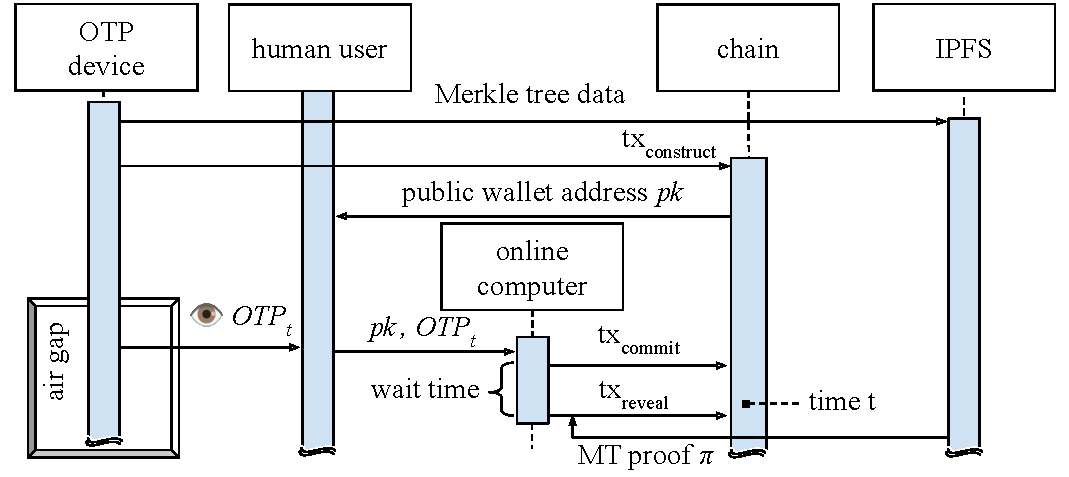
\includegraphics[width=\textwidth,keepaspectratio]{figures/otp-sequence-diagram.pdf}
    \else
        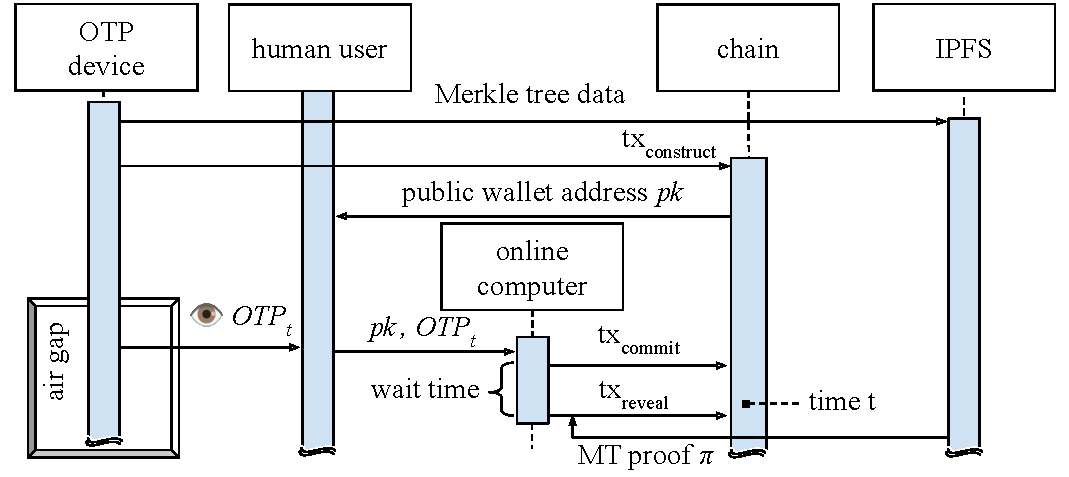
\includegraphics[width=0.7 \textwidth,keepaspectratio]{figures/otp-sequence-diagram.pdf}
    \fi
    \label{fig.sequence-diagram}
\end{figure*}

\section{An OTP Wallet}

The password-based construction has an important limitaton:
The money can only be spent once at a prespecified date. This makes
the wallet unusable.
Using the previous construction as a stepping stone,
we now move on to describe our \emph{Hours of Horus} scheme.
This is an OTP-based scheme in which the OTP is used as the \emph{single factor}
for wallet access, without any need of private keys.

The workflow of the OTP wallet is illustrated as a sequence diagram
in Figure~\ref{fig.sequence-diagram}. At the beginning, Alice initializes
a time-based OTP device (such as a mobile phone app) which
generates and stores an OTP seed (leftmost column). Upon this generation, the device also
generates a smart contract, which is constructed and submitted to the chain
through a transaction $\textsf{tx}_\textsf{construct}$.
This transaction generates a wallet address $pk$ to which
payers can send money for Alice. The OTP device also constructs a Merkle tree containing
a large number of encrypted future OTPs and submits them to IPFS~\cite{ipfs} (or other persistent storage service)
publicly for availability (rightmost column).
Both $pk$ and all internal Merkle tree nodes are public. After this
initial phase, the OTP device becomes air gapped.

At any time Alice wishes to spend, she visually consults her OTP device which displays a time-based
OTP key. Using a (newly booted) online computer, she creates a transaction $\textsf{tx}_\textsf{commit}$ in
which she commits to the $OTP$, the amount she wishes to spend, and the target address.
The wallet waits a short amount of time before submitting the final $\textsf{tx}_\textsf{reveal}$
to confirm the spending. This transaction is accompanied by a Merkle tree proof-of-inclusion
constructed using the IPFS data. The wallet then releases the payment to the desired address.

\begin{figure}[H]
    \caption{Each $\textsf{OTP}_t$ is timelocked with time $t$. All timelock
             ciphertexts $c_t$ are
             organized into a Merkle Tree whose root is $r$.}
    \centering
    \iftwocolumn
        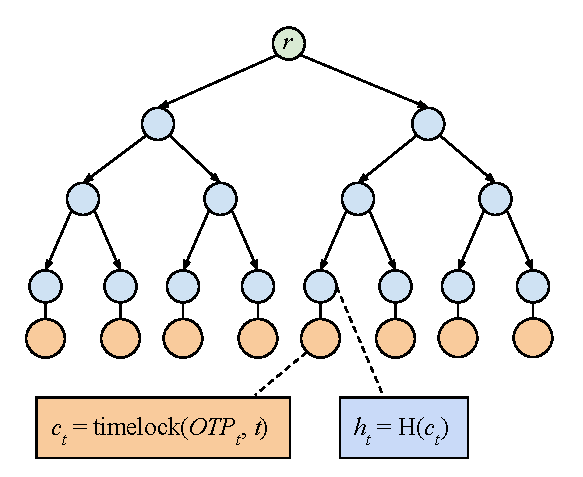
\includegraphics[width=\columnwidth,keepaspectratio]{figures/timelock-merkle.pdf}
    \else
        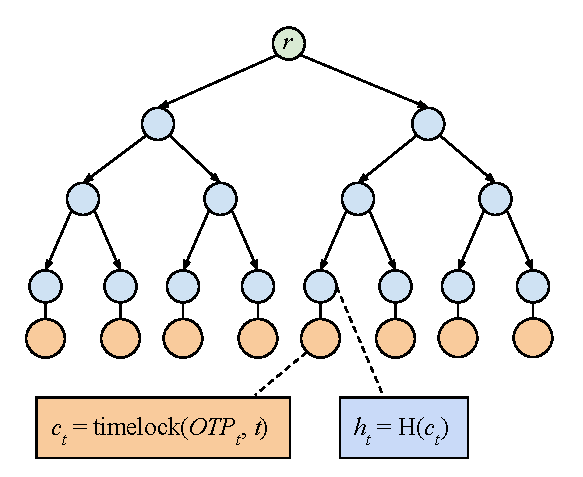
\includegraphics[width=0.6 \columnwidth,keepaspectratio]{figures/timelock-merkle.pdf}
    \fi
    \label{fig.merkle-otp}
\end{figure}

The contract deployed as a wallet is illustrated in Algorithm~\ref{alg.otp}.
The interaction with the contract by the user is illustrated in Algorithm~\ref{alg.otp.external}.
The constructor accepts a parameter $r$
denoting a Merkle tree root. This is constructed by generating a large number ($\textsf{MAX\_TIME}$)
of time-based OTPs for the foreseeable future. For example, to support a wallet with
a lifetime of $100$ years with an hourly OTP resolution, $876{,}000$ codes need to
be generated. Let ${OTP}_t$ denote the OTP for future time $t \in \mathbb{N}$ (in
the example, $t$ ranges from $1$ to $876{,}000$). These are generated from
the OTP seed in the OTP device by invoking the pseudorandom function
$\mathcal{G}(\textsf{seed}, t)$ whose output has $\lambda$ bits of entropy.
Each such OTP is then timelock encrypted for time $t$, multiplied by the expected
hourly production rate of the blockchain (the \emph{hourly} resolution is an arbitrary
choice that can be made differently, giving rise to a tradeoff between how much
data must be stored on IPFS versus how often the user can spend her money).
Specifically, the software computes $c_t = \textsf{timelock}(\textsf{OTP}_t, t)$,
(setting $c_t = \textsf{WE.Enc}_\mathcal{R}(\textsf{OTP}_t, x)$, where $x = (B, t)$).
All of these $c_t$ are then organized into a Merkle tree as illustrated in
Figure~\ref{fig.merkle-otp}
using the hash function $H$ whose root is $r$. This $r$ is submitted
to the constructor.

\import{./}{algorithms/alg.otp.tex}
\import{./}{algorithms/alg.otp.external.tex}

When Alice wishes to spend, she calls \emph{commit} by issuing a
$\textsf{tx}_\textsf{commit}$ transaction. The
method takes parameters $z$ and $t$. Here, $z$ is the commitment
$z = H(\left<\textsf{OTP}, \textsf{salt}, \alpha_{\textsf{to}}, \textsf{amount}\right>)$.
For $t$, Alice looks at her local chain $\chain$, obtains its length $|\chain|$
and evaluates $t = |\chain| + \ell + 2k$.
So, $t$ is a block height at least $\ell + 2k$ blocks in the future.
As liveness ensures this transaction will confirm within $\ell$ blocks,
the condition on Line~\ref{alg.otp.delay} will succeed.
The contract records the pair $(z, t)$ in the \emph{commitments} set.
Alice waits for her chain to grow to a height of $t$ blocks,
at which point she issues the $\textsf{tx}_\textsf{reveal}$ transaction
calling the \emph{reveal} method. She reveals
the OTP (no longer useful to any adversary), the salt,
the destination address, and the amount to transfer. These are accompanied
by proof-of-inclusion $\pi$ at position $t$ in the Merkle Tree whose root $r$
is recorded in the contract obtained from the data stored on IPFS
(anyone can compute this). Additionally, it is accompanied by a witness that
time $t$ has passed by providing the chain portion $\chain\{B{:}\}$ (this can
also be computed by anyone). The contract verifies the provided
data are included in previous commitments, that the Merkle tree proof is
valid for the specified position, and that the timelock encryption of the
provided OTP corresponds to the given ciphertext.

The honest party will always succeed in creating a valid spending transaction.
To see this, note that the party begins creating the commit transaction at time
$t - \ell - 2k$. Due to liveness, it becomes confirmed at block $t - 2k$ at most,
and so the check in Line~\ref{alg.otp.delay} will pass. The reveal transaction will
be called with the corresponding data and release the funds.

To see why an adversary cannot create a valid spending transaction beyond random
guessing, we note that any adversary can either provide a commit transaction prior
to block $t - 2k$, or afterwards. If she provides it
prior, then the timelock scheme will protect the secret, and so the spending
transaction will include a random OTP guess. On the other hand, if she provides it
afterwards, it will not be accepted due to the time delay enforced
in Line~\ref{alg.otp.delay}. Consult the Analysis section for a more complete argument.
